\begin{figure}[htbp]\centering
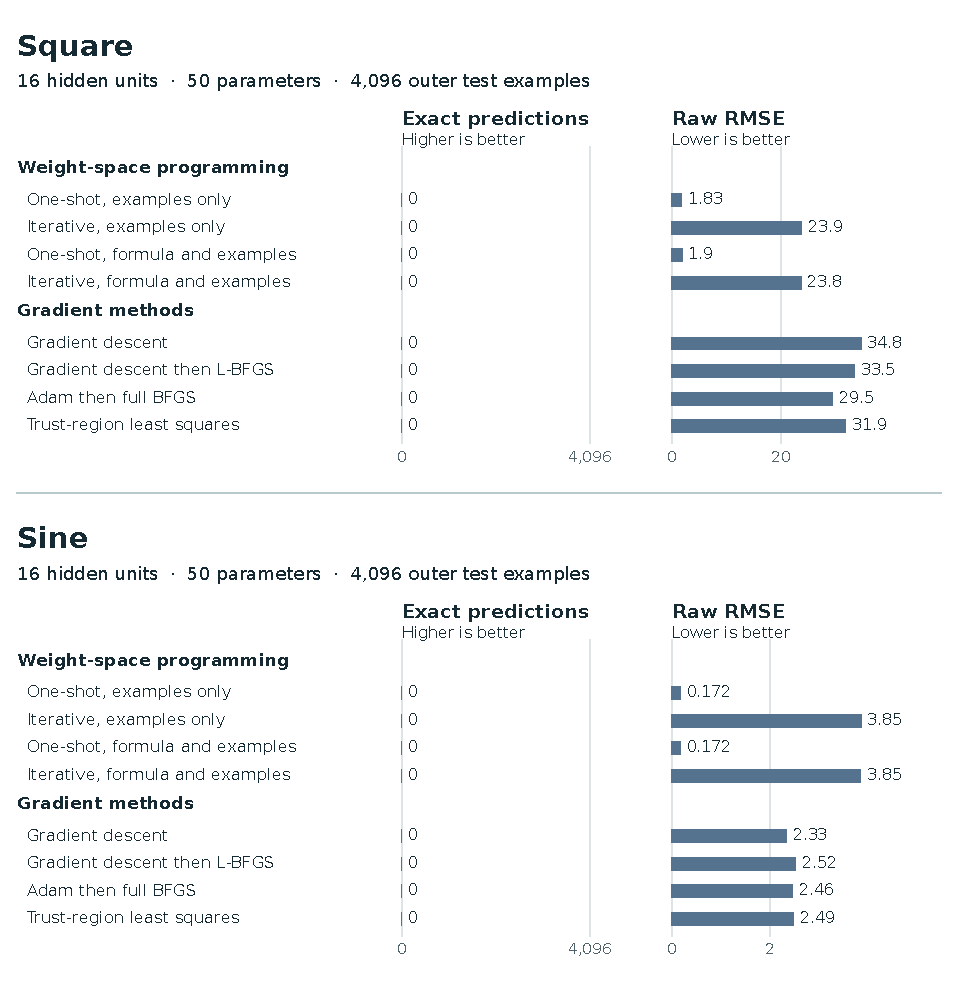
\includegraphics[width=\linewidth]{task_panels_1.pdf}
\caption{Square and sine on the extrapolation test at the sizes in Table~\ref{tab:focusouter}. Bars show medians over three starts. Exact predictions count whole examples that match the reference. Raw root mean squared error (RMSE) is in the target's units. Each task has its own linear error axis starting at zero.}
\label{fig:taskbars1}
\end{figure}
\begin{figure}[p]\centering
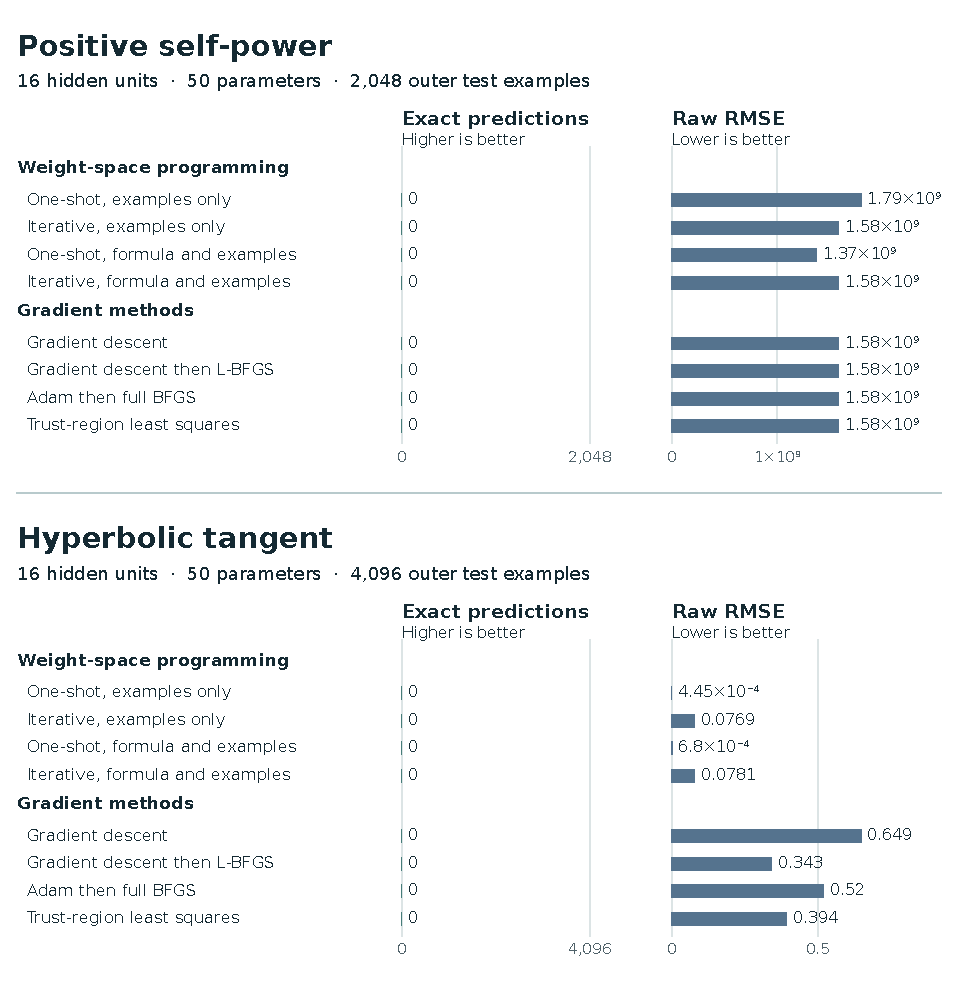
\includegraphics[width=\linewidth]{task_panels_2.pdf}
\caption{Positive self-power and hyperbolic tangent on the extrapolation test at the sizes in Table~\ref{tab:focusouter}. Bars show medians over three starts. Exact predictions count whole examples that match the reference. Raw root mean squared error (RMSE) is in the target's units. Each task has its own linear error axis starting at zero.}
\label{fig:taskbars2}
\end{figure}
\begin{figure}[p]\centering
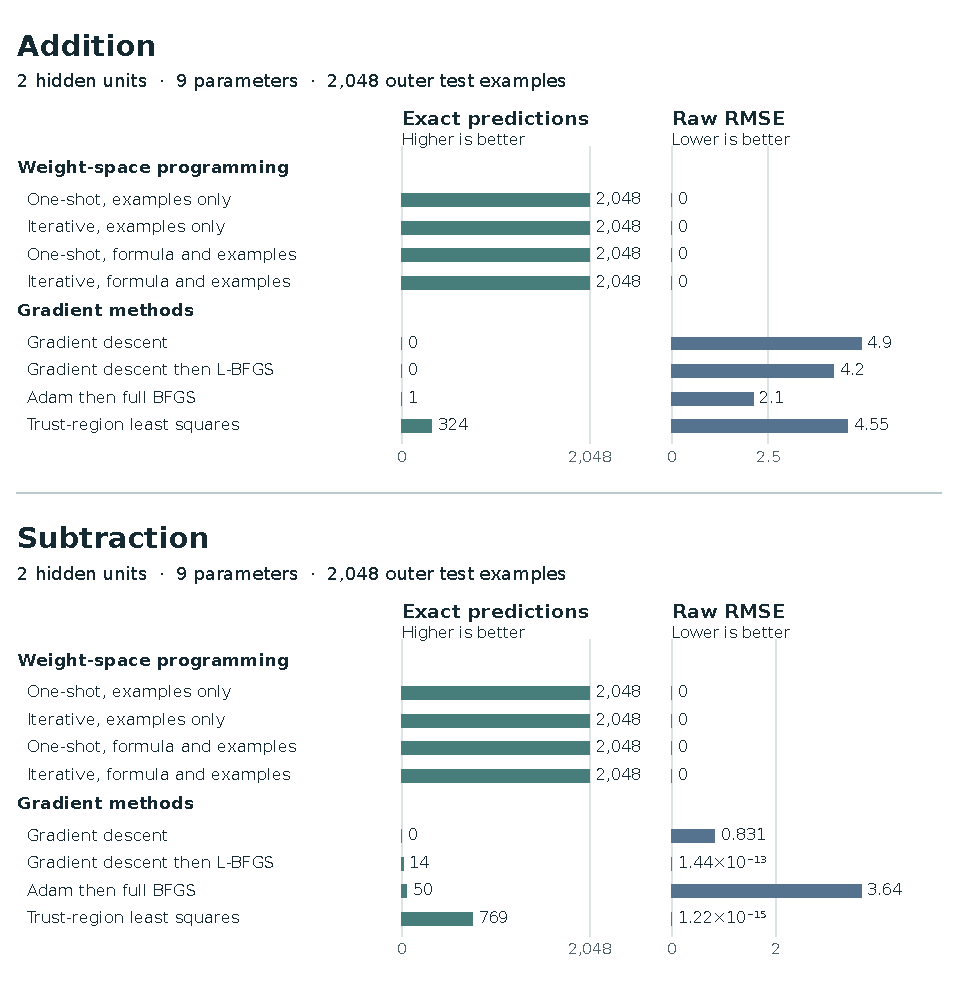
\includegraphics[width=\linewidth]{task_panels_3.pdf}
\caption{Addition and subtraction on the extrapolation test at the sizes in Table~\ref{tab:focusouter}. Bars show medians over three starts. Exact predictions count whole examples that match the reference. Raw root mean squared error (RMSE) is in the target's units. Each task has its own linear error axis starting at zero.}
\label{fig:taskbars3}
\end{figure}
\begin{figure}[p]\centering
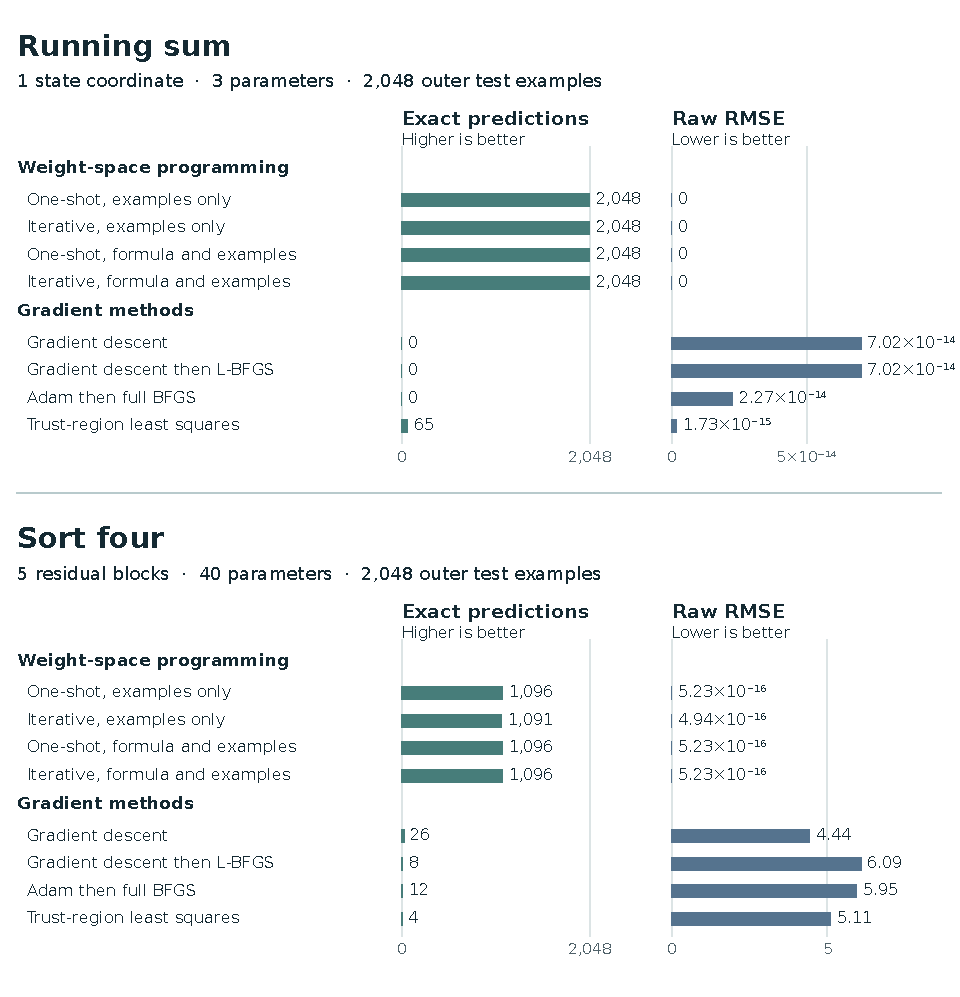
\includegraphics[width=\linewidth]{task_panels_4.pdf}
\caption{Running sum and sort four on the extrapolation test at the sizes in Table~\ref{tab:focusouter}. Bars show medians over three starts. Exact predictions count whole examples that match the reference. Raw root mean squared error (RMSE) is in the target's units. Each task has its own linear error axis starting at zero.}
\label{fig:taskbars4}
\end{figure}
\begin{figure}[p]\centering
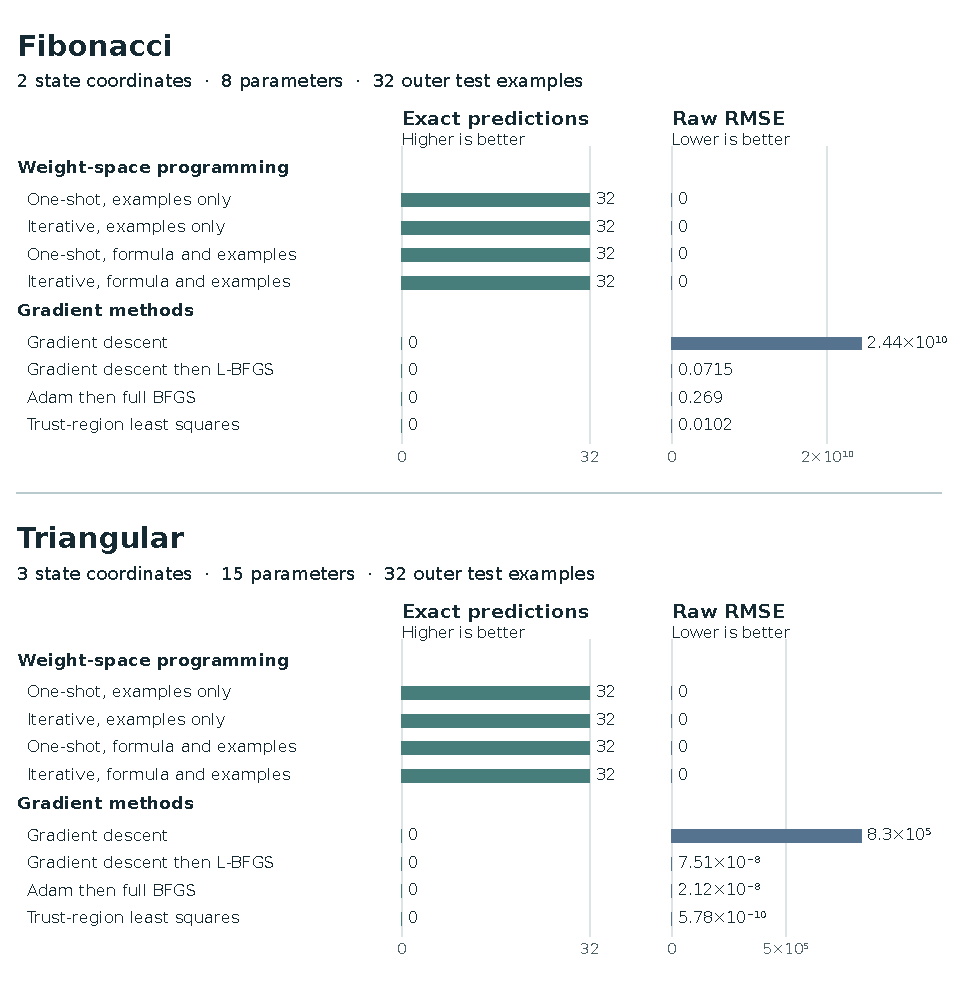
\includegraphics[width=\linewidth]{task_panels_5.pdf}
\caption{Fibonacci and triangular on the extrapolation test at the sizes in Table~\ref{tab:focusouter}. Bars show medians over three starts. Exact predictions count whole examples that match the reference. Raw root mean squared error (RMSE) is in the target's units. Each task has its own linear error axis starting at zero.}
\label{fig:taskbars5}
\end{figure}
\clearpage
